\documentclass[svgnames,11pt]{beamer}
\input{/home/tof/Documents/Cozy/latex-include/preambule_commun.tex}
\input{/home/tof/Documents/Cozy/latex-include/preambule_beamer.tex}
%\usepackage{pgfpages} \setbeameroption{show notes on second screen=left}
\author[]{Christophe Viroulaud}
\title{TP Terminus}
\date{\framebox{\textbf{ArchMat 10}}}
%\logo{}
\institute{Première - NSI}

\begin{document}
\begin{frame}
\titlepage
\end{frame}
\begin{frame}
    \frametitle{}

    Nous avons l'habitude d'interagir avec le système d'exploitation grâce à son interface graphique (bureau, explorateur\dots). Il reste cependant pertinent de savoir utiliser les commandes \emph{en mode console} lors de l'intervention sur un serveur à distance par exemple.

\end{frame}
\begin{frame}
    \frametitle{}

    \begin{framed}
        \centering Quelles commandes principales permettent d'interagir avec le système d'exploitation?
    \end{framed}

\end{frame}
\section{Commandes de base}
\subsection{Les répertoires}
\begin{frame}
    \frametitle{Commandes de base - Les répertoires}

    Pour interagir avec le système de fichiers, il faut le connaître:

\begin{center}
\centering

\includegraphics[width=7.5cm]{ressources/arbre-linux.png}
\captionof{figure}{\centering Arborescence simplifiée d'un système Linux.}
\label{IMG}
\end{center}
\end{frame}
\begin{frame}
    \frametitle{}

    \begin{aretenir}[]
    \begin{itemize}
        \item Toutes les distributions Linux ont la même structure.
        \item Le répertoire racine se nomme \textbf{\texttt{/}}
        \item Chaque utilisateur possède un répertoire personnel, situé dans \textbf{\texttt{home}}. Il y a, dans l'exemple, deux utilisateurs: max et elsa.
        \item Le répertoire personnel est le seul accessible en écriture pour l'utilisateur.
        \item Il faut passer super-utilisateur pour modifier un autre répertoire.
    \end{itemize}
    \end{aretenir}

\end{frame}
\begin{frame}[fragile]
    \frametitle{}

\begin{center}
\begin{lstlisting}[language=Bash , basicstyle=\ttfamily\small, xleftmargin=1em, xrightmargin=1em]
# Afficher le chemin absolu du répertoire
pwd

# Lister le contenu d'un répertoire
ls

# Créer un répertoire
mkdir mon_repertoire

# Se déplacer dans les répertoires
cd nom_repertoire
\end{lstlisting}
\captionof{code}{\centering Quelques commandes pour travailler avec les répertoires.}
\end{center}

\end{frame}
\begin{frame}
    \frametitle{}

    \begin{activite}
    \begin{enumerate}
        \item Ouvrir la machine virtuelle.
        \item Ouvrir un \textbf{terminal}.
    \end{enumerate}
    \end{activite}

\end{frame}
\begin{frame}[fragile]
    \frametitle{}

\begin{center}
\begin{lstlisting}[language=Python , basicstyle=\ttfamily\small, xleftmargin=2em, xrightmargin=2em]
le_boss@mon_beau_pc:~$
\end{lstlisting}
\captionof{code}{Exemple de l'invite d'un terminal.}
\label{CODE}
\end{center}
\textbf{L'invite de commande} affiche plusieurs informations:
\begin{itemize}
    \item L'utilisateur se nomme \emph{le\_boss},
    \item la machine se nomme \emph{mon\_beau\_pc},
    \item le terminal s'ouvre par défaut dans le dossier de l'utilisateur:
    \begin{itemize}
        \item Son adresse est \textbf{\texttt{/home/le\_boss}}.
        \item On peut y accéder par le raccourci \textbf{\texttt{~}}
    \end{itemize}
\end{itemize}
\end{frame}
\begin{frame}
    \frametitle{}

    \begin{activite}
    \begin{enumerate}
        \item Afficher le chemin du répertoire courant.
        \item Afficher le contenu du répertoire.
        \item Créer le répertoire \textbf{\texttt{mon\_test}}
        \item Entrer dans le répertoire nouvellement crée.
    \end{enumerate}
    \end{activite}

\end{frame}
\begin{frame}
    \frametitle{Avant de regarder la correction}
\begin{center}
    \centering
    \includegraphics[width=3cm]{/home/tof/Documents/Cozy/latex-include/stop.png}
    \end{center}
{\Large
    \begin{itemize}
        \item Prendre le temps de réfléchir,
        \item Analyser les messages d'erreur,
        \item Demander au professeur.
    \end{itemize}
}
\end{frame}
\begin{frame}[fragile]
    \frametitle{}

\begin{center}
\begin{lstlisting}[language=Python , basicstyle=\ttfamily\small, xleftmargin=2em, xrightmargin=2em]
pwd
ls
mkdir mon_test
cd mon_test
\end{lstlisting}
\captionof{code}{Nouveau répertoire.}
\end{center}
\begin{center}
\begin{lstlisting}[language=Python , basicstyle=\ttfamily\small, xleftmargin=2em, xrightmargin=2em]
cd ..
\end{lstlisting}
\captionof{code}{Pour revenir dans le répertoire précédent.}
\label{CODE}
\end{center}
\end{frame}
\subsection{Les fichiers}
\begin{frame}[fragile]
    \frametitle{Les fichiers}

Un répertoire peut contenir d'autres répertoires mais également des \textbf{fichiers}.
\begin{activite}
\begin{enumerate}
    \item Créer un fichier texte avec la commande:
\begin{lstlisting}[language=Python , basicstyle=\ttfamily\small, xleftmargin=2em, xrightmargin=2em]
cat > mon_fichier.txt
\end{lstlisting}
\item Remplir le fichier avec plusieurs lignes. Appuyer sur \textbf{\texttt{Entrée}} pour revenir à la ligne.
\item Quitter le fichier avec le raccourci \textbf{\texttt{ctrl + D}}
\item Lire le contenu du fichier avec la commande:
\begin{lstlisting}[language=Python , basicstyle=\ttfamily\small, xleftmargin=2em, xrightmargin=2em]
cat mon_fichier.txt
\end{lstlisting}
\item Ajouter des éléments à la fin du fichier avec:
\begin{lstlisting}[language=Python , basicstyle=\ttfamily\small, xleftmargin=2em, xrightmargin=2em]
cat >> mon_fichier.txt
\end{lstlisting}
\end{enumerate}
\end{activite}

\end{frame}
\begin{frame}[fragile]
    \frametitle{}

    \begin{activite}
    \begin{enumerate}
        \item Afficher le contenu détaillé du répertoire avec la commande:
\begin{lstlisting}[language=Python , basicstyle=\ttfamily\small, xleftmargin=2em, xrightmargin=2em]
ls -lh
\end{lstlisting}
\item En début de ligne, repérer ce qui distingue les fichiers des répertoires. 
    \end{enumerate}
    \end{activite}

\end{frame}
\begin{frame}
    \frametitle{Avant de regarder la correction}
\begin{center}
    \centering
    \includegraphics[width=3cm]{/home/tof/Documents/Cozy/latex-include/stop.png}
    \end{center}
{\Large
    \begin{itemize}
        \item Prendre le temps de réfléchir,
        \item Analyser les messages d'erreur,
        \item Demander au professeur.
    \end{itemize}
}
\end{frame}
\begin{frame}[fragile]
    \frametitle{}
\begin{center}
\begin{lstlisting}[language=Python , basicstyle=\ttfamily\small, xleftmargin=1em, xrightmargin=0em]
drwxr-xr-x  9 tof tof  20K mai   12 22:52  Cours
-rw-r--r--  1 tof tof    3 mai   13 09:05  test
\end{lstlisting}
\end{center}
    
\begin{aretenir}[]
Le \textbf{\texttt{d}} en début de ligne signifie \textbf{directory (répertoire)}.

NB: les lettres suivantes évoquent les droits des utilisateurs sur les fichiers ou répertoires.
\end{aretenir}
\end{frame}
\section{Jeu sérieux}
\begin{frame}
    \frametitle{Jeu sérieux}

    Pour mémoriser les commandes, il faut manipuler encore et encore. Le jeu sérieux \textbf{Terminus} propose de s'entraîner à travers une petite aventure. L'objectif est de parcourir les salles (les répertoires), interagir avec les personnages ou les objets (les fichiers), réaliser des sorts (les commandes).

\end{frame}
\begin{frame}
    \frametitle{}

    \begin{activite}
        \begin{enumerate}
            \item Se rendre sur \url{http://luffah.xyz/bidules/Terminus/}
            \item Commencer le jeu en entrant un nom et en validant.
            \item Au fur et à mesure de l'avancement dans la partie, maintenir sur une feuille (modèle page suivante):
            \begin{itemize}
                \item un plan du jeu (figure \ref{modele}),
                \item un tableau des commandes et leur utilité (figure \ref{tab}).
            \end{itemize}
        \end{enumerate}
        \end{activite}

\end{frame}
\begin{frame}
    \frametitle{}

    
\begin{center}
    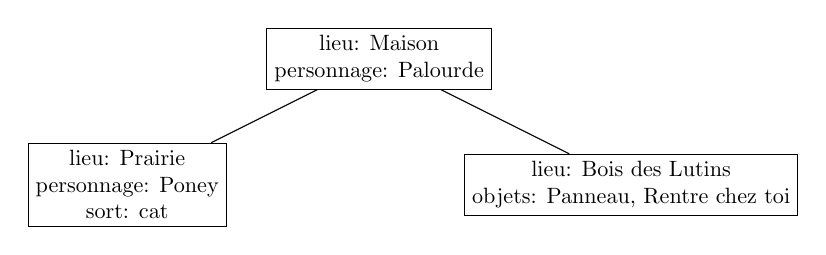
\begin{tikzpicture}[scale=0.8,transform shape, every text node part/.style={align=center}]
    \node[rectangle, draw] (A) at (0,0) {lieu: Maison \\ personnage: Palourde};
    \node[rectangle, draw] (B) at (-4,-2) {lieu: Prairie \\ personnage: Poney \\ sort: cat};
    \node[rectangle, draw] (C) at (4,-2) {lieu: Bois des Lutins \\ objets: Panneau, Rentre chez toi};
    
    \draw (A)--(B);
    \draw (A)--(C);
    \end{tikzpicture}
    \captionof{figure}{Modèle de plan}
    \label{modele}
    \end{center}
    \begin{center}
        \begin{tabular}{|*{3}{c|}}
            \hline
            commande & description & utilisation dans le jeu \\
            \hline
            cat & Examiner en détail & Interagir avec un objet\\
            \hline
        \end{tabular}
        \captionof{figure}{Exemple de tableau}
        \label{tab}
    \end{center}
\end{frame}
\end{document}